\documentclass[12pt]{article}
\usepackage{graphicx}
\usepackage{subcaption}
\setlength{\parindent}{0pt}
\setlength{\parskip}{10pt} % block paragraphs
\begin{document}

\title*{\centerline{\huge{CAP 5619 \-- Deep and Reinforcement Learning}}}
\author*{\centerline{Homework 1 Hua Huang}}%unnumbered centered head

In this homework, the example of mnist\_mlp.py from Keras tutorial is
used. It is slightly modified in solving problem 2.
\section{Problem 1}
(1) It's a MLP network, in which there is 4 layers, namely input layer, 2 hidden
 layers, and output layer. The 2 hidden layers have Re\--LU non\--linear units,
the output layer has softmax activation function. The input is a 784 dimension 
vector, two hidden layers are of dimension 512, output layer has 10 units.
In total, there are $(784+1)\times 512+(512+1)\times 512+(512+1)\times 10=669706$ parameters.\\
(2)
\begin{figure}[h]
    \centering
    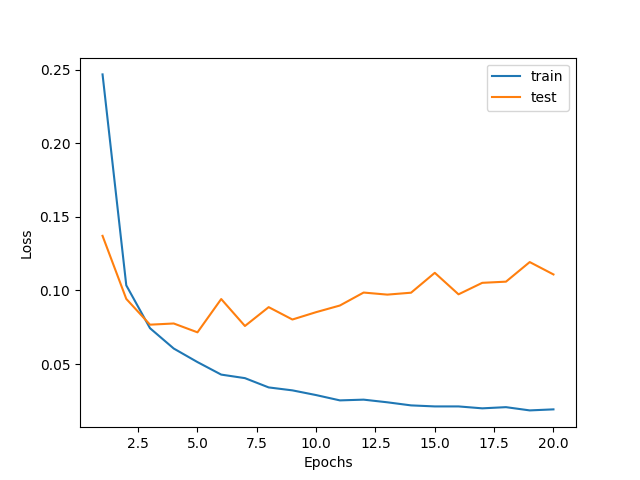
\includegraphics [scale=0.5]{Figure_0.png}
    \caption {Loss}
\end{figure}
\begin{figure}[h]
    \centering
    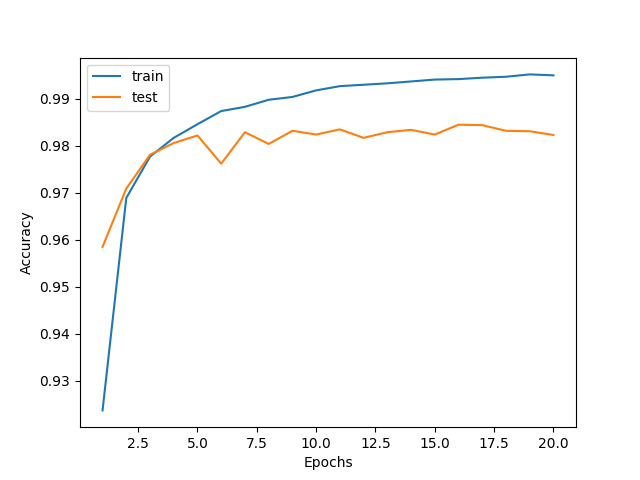
\includegraphics [scale=0.5]{Figure_1.png}
    \caption {Accuracy}
\end{figure}
\newpage

\section{Problem 2}
(1) Here in the training, the labels are changed to random numbers from
$0\sim9$. Since the training is much slower then in problem 1, here
epochs are increased to 200.\\
\begin{figure}[h]
    \centering
    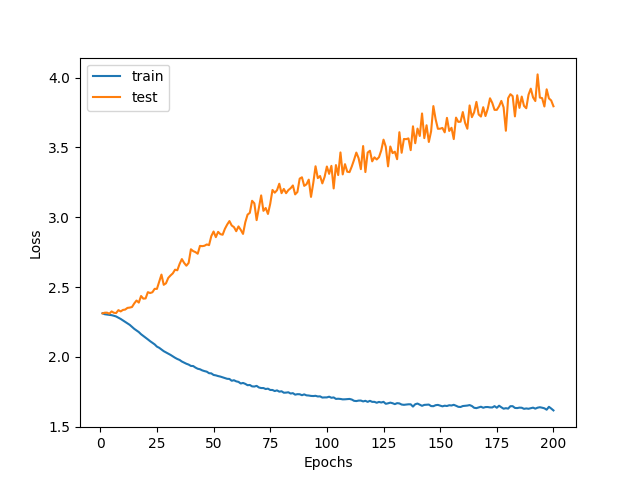
\includegraphics [scale=0.5]{Figure_2.png}
    \caption {Loss}
\end{figure}
\begin{figure}[h]
    \centering
    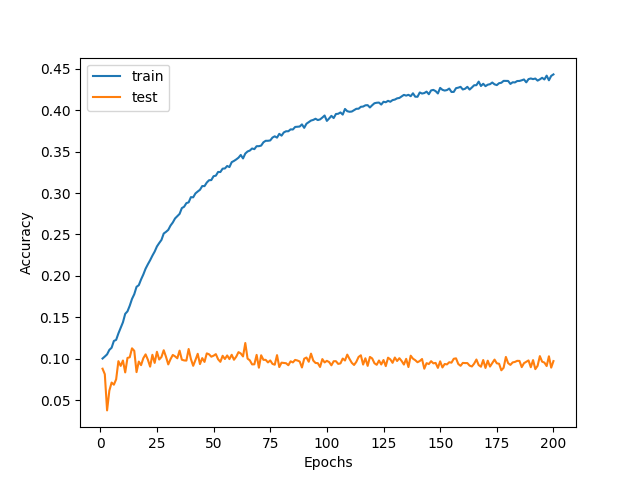
\includegraphics [scale=0.5]{Figure_3.png}
    \caption {Accuracy}
\end{figure}
(2) One of the biggest difference is the randomized lables in training
dramatically slower the trainning process. Interestingly, it's
reasonable to speculate if we increase the total epochs further, say
1000 epochs, we might still get a near\--perfect training accuracy. 
Just as expected, the test accuracy is just the probalbility of being
the actual labels when random number is picked uniformly from $0\sim9$,
namely $0.1$. This leads to a significantly increased gap between the
training and test accuracy.\\
The difference may be introduced by the fact that deep neural network
is so powerful in representation, that it can "remeber" the training
data (here is the pixels in training data) if we train the training
data long enough. This "remeber" is not learning, namely it will not be
able to generalize to data it never seen before, so it will not be able 
to predict the test data, eventually we see a huge gap in the accuracy
of traing data and test data.

\section{Problem 3}
The paper indicates the difficulty in explaning the generalization
capability of deep network. If we want to improve the generalization 
capability, namely reduce the gap between training accuracy and test
accuracy, regularization may or may not work. In this test, dropout is
added but it failed to reduce the gap.\\
Thanks to this assignment, now I can understand why \textbf{early stop} will
help reduce over\--training and improve generalization. Deep neural
network is so powerful it can easily memorize the trianing data, and
this memorizing is not learning, it will not be able to predict the
data it never seen.
\end{document}


